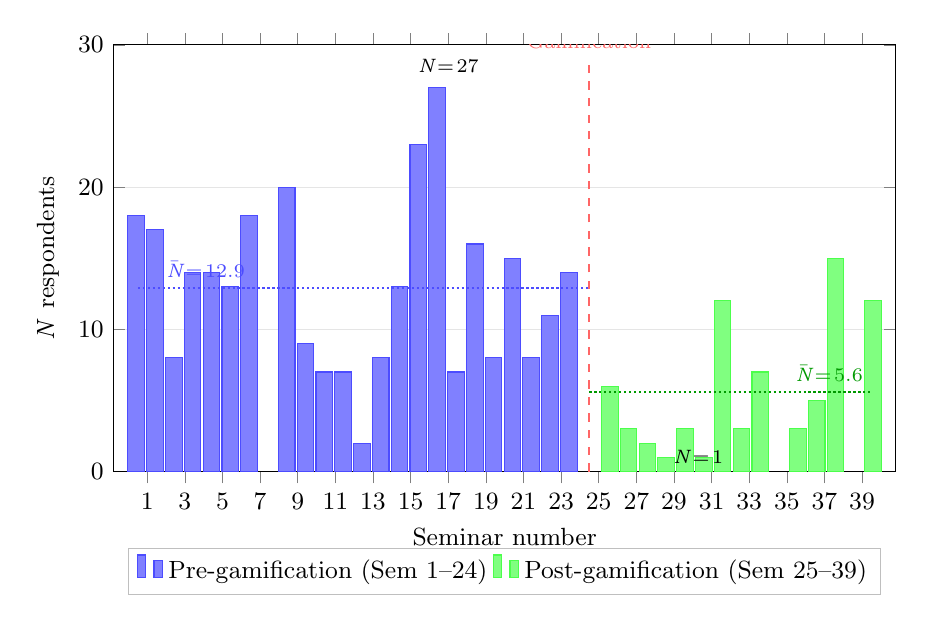
\begin{tikzpicture}
\begin{axis}[
  ybar,
  width=0.95\textwidth,
  height=7cm,
  bar width=6pt,
  ylabel={\textit{N} respondents},
  xlabel={Seminar number},
  ymin=0, ymax=30,
  xtick={1,3,5,7,9,11,13,15,17,19,21,23,25,27,29,31,33,35,37,39},
  xmin=0, xmax=40,
  enlarge x limits=0.02,
  legend style={at={(0.5,-0.18)}, anchor=north, legend columns=2, font=\small, draw=gray!50},
  ymajorgrids=true,
  grid style={gray!20},
  tick label style={font=\small},
  label style={font=\small},
]

% Pre-gamification bars (blue)
\addplot[fill=blue!50, draw=blue!70] coordinates {
  (1,18) (2,17) (3,8) (4,14) (5,14) (6,13) (7,18)
  (9,20) (10,9) (11,7) (12,7) (13,2) (14,8) (15,13)
  (16,23) (17,27) (18,7) (19,16) (20,8) (21,15) (22,8) (23,11) (24,14)
};

% Post-gamification bars (green)
\addplot[fill=green!50, draw=green!70] coordinates {
  (25,6) (26,3) (27,2) (28,1) (29,3) (30,1)
  (31,12) (32,3) (33,7) (35,3) (36,5) (37,15) (39,12)
};

\legend{Pre-gamification (Sem 1--24), Post-gamification (Sem 25--39)}

% Gamification boundary
\draw[dashed, thick, red!60] (axis cs:24.5,0) -- (axis cs:24.5,29)
  node[above, font=\scriptsize, red!60] {Gamification};

% Period mean lines
\draw[densely dotted, blue!70, thick] (axis cs:0.5,12.9) -- (axis cs:24.5,12.9)
  node[pos=0.15, above, font=\scriptsize, blue!70] {$\bar{\textit{N}}\!=\!12.9$};
\draw[densely dotted, green!60!black, thick] (axis cs:24.5,5.6) -- (axis cs:39.5,5.6)
  node[pos=0.85, above, font=\scriptsize, green!60!black] {$\bar{\textit{N}}\!=\!5.6$};

% Annotations
\node[font=\scriptsize, above, yshift=2pt] at (axis cs:17,27) {$\textit{N}\!=\!27$};
\node[font=\scriptsize, right, xshift=3pt] at (axis cs:28,1) {$\textit{N}\!=\!1$};

\end{axis}
\end{tikzpicture}
